% \begin{quotation}
% This program is free software: you can redistribute it and/or modify
% it under the terms of the GNU General Public License as published by
% the Free Software Foundation, either version 3 of the License, or
% (at your option) any later version.

% This program is distributed in the hope that it will be useful,
% but WITHOUT ANY WARRANTY; without even the implied warranty of
% MERCHANTABILITY or FITNESS FOR A PARTICULAR PURPOSE.  See the
% GNU General Public License for more details.

% You should have received a copy of the GNU General Public License
% along with this program.  If not, see <http://www.gnu.org/licenses/>.
% \end{quotation}

% Author: Chel Hee Lee
% Created on 2013-APR-11
% Modified on 2013-APR-11

% The HTML syntax generated from this document will be added to the page
% ./ihelp/www/sk_tips.html
% htlatex $(file_name).tex "html, 4, mouseover, frames, next" "" "-dweb/"
% htlatex tips.tex "html, 1, mouseover, next"

% graphics file must be in the format of .eps

% 아 안된다... tex에서 한글사용 어렵다.... 

% fullpage.sty 파일이 없다는 에러가 나옵니다.. 해결 방법은?

% R은 처음부터 기존의 통계팩키지와는 다른 모습에 약간 두렵기까지 하다..
% 기존의 분석은 일반적으로 [프로그램 실행 -> 데이터 불러오기 -> 분석(메뉴클릭:SPSS 또는 명령어입력:SAS) -> 실행]의 절차를 밟아왔다.
% 즉 할 거 다하고 나중에 결과를 보는 식이다.
% 그러나 R은 다르다. 일단 여기부터 생소하다.
% 뭔가 이상하다.. 하는 거 같은 느낌도 없다. 데이터를 불러오기 하면 바로 데이터시트를 볼 수 있는 것도 아니다.
% 물론 나중에는 스크립트를 이용하여 비슷한 방법으로 분석을 실행할 수도 있음을 알게 되었지만 이것도 친숙한 편은 아니다.
% 이런 느낌은 특히 최소한 내가 알기로는 경영학과 경제학 분야(거의 확실함) 및 사회학, 심리학 분야가 특히 심하다. 그리고 이들 분야에서는
% R의 다양한 기능(특히 visualization) 또는 packages를 필요로 하지 않을 가능성이 높다. 왜냐하면 분석 방법이 단순하기 때문이다.
% 여기에서 분석 방법이 단순하다는 것은 그 이론적 배경이 쉽다는 것을 의미하는 것이 아니라 절차상의 얘기이다.
% 언급한 분야에서 학술연구에서 실행되는 분석의 양을 보면 대부분 [기술통계 - 상관관계 - 차이분석, 회귀분석, 구조방정식분석] 정도로
% 분석이 마무리 되기 때문이다. 그리고 대부분 표(table)로 결과를 보고하는 형식을 따르고 있다. 
% 분석 모형 자체를 다루는 연구가 거의 없는 것이다. 따라서 R의 작업 방식은 그들에게는 불필요할 지도 모른다.

% 그러나 여전히 R의 다양한 source를 필요로 하는 아주 작은 규모의 학술연구 분야는 존재한다. 따라서 여기의 tips에는 이들을 고려하여
% R 사용에 도움이 될 만한 사항들을 정리하고자 한다.
% 개인적으로는 통계학 및 다른 분야의 연구 과정이 어떻게 진행되는지 잘 모르는 것도 한 몫하여 이에 해당하는 부분은 다른 이의 도움이 
% 절실하다.

% 덧붙여 나는 윈도우 환경에서의 R tip에 주목하고자 한다(Mac이나 유닉스/리눅스 환경에서의 R 사용에 관한 tip도 다른 이의 도움이 필요한
% 부분이다). 그 이유는 내가 윈도우에서 SPSS와 SAS를 숙련시켜 왔기 때문에 대부분의 통계분석 초심자들도 윈도우 환경에서 R을 접하게
% 될 것이라는 막연한 억측 때문이다. 시간이 지나면서 여러 사람들을 만나보게 꼭 그렇지만은 않다는 것을 알게 되었지만 최소한 경영학과
% 경제학 분야에 속한 사람들은 그럴 것이라는 확신 때문이다. 이것은 다른 분야의 사람들을 홀대하는 것이 아니라 나의 능력의 한계 때문이다.
% 실제로 나의 경우에도 최근에 C 언어, CentOS, 그리고 MySQL도 공부하기 시작했으니 오해는 하지 말기 바란다(누군가는 포기하라고도 했다.
% 왜냐하면 지금 그것들을 공부하기에는 분량이 너무 많고 난이도가 낮지 않기 때문이다). 그런데 결국에는 내 전공분야에서의 R 사용은 
% 그 분량이 많지 않고 리눅스/유닉스 기반의 R 사용에 보다 많은 시간과 지면을 할애하게 될 것이라는 생각이 든다.

% R은 최근의 빅데이터라는 화두와 함께 큰 주목을 받고 있다. 하지만 대부분의 사람들, 특히 사회과학 전공자들은 이 개념적 정의도 제대로
% 알지 못하며 들어보지 못한  전문용어(SQL, Hadoop, 그리고 Mapreduce 등)에 혹하고 있는 실정이다.
% 나의 경우 R을 구글링(googling)으로 공부하였다. 왜냐하면 내가 재학하던 대학에서는 R 교육 프로그램이 없었기 때문이다. 처음 접하게 된 
% 것은 미시경제분석 수업이었다. 그 수업에서 교수님이 수업을 진행하시는데 R을 사용한 것이다(SAS도 조금 사용했었으나 SPSS는 잡동사니
% 취급을 하셨던 것으로 기억한다). 누군가에게 강의를 받는 식의 교육은 그것이 전부였다. 이후의 학습은 모두 맨땅에 해딩과 계란으로 
% 바위깨기 식이었다. 이 R tips 과정은 이러한 어려움을 덜어주기 위한 방안이 될 수도 있을 것이다.
% 그러기를 한참 후 어느 정도 익숙해지고 나니, 또 연구자로서의 건방이 살아나 R 교육이 어떻게 이루어지고 있는 지가 궁금해졌다.
% 이 부분은 나중에 다시 써 볼라오,,,


\documentclass{article}

\usepackage{mystyle}
% \usepackage{kotex, url, hyperref, Sweave}

\title{Some R Problems Derived Me Nuts Before!}
\author{iHELP Working Group \\ Chel Hee Lee \& Eugene Jung}

\begin{document}
\maketitle

\paragraph{읽기전에:}
\texttt{R}을 사용하게 된 이래로 경험하게 된 여러가지 팁들을 정리한 것입니다.
% \textsf{본 페이지의 작성자는 다른 사용자들이 사용하는 놀라운 테크닉을 항상 배우고 있습니다}.
% 이 문서는 매일 하루에 하나의 팁이 올라올 수 있도록 노력할 예정입니다.


% 실제로 R을 처음 접한 사람들은 
% > library()
% 의 사용도 자각하지 못하는 경우가 많다.
% 그래서 초기에 가장 많이 보는 에러가 [---함수가 없습니다.] 또는 [---함수를 찾을 수 없습니다.]이다.
% package를 사용하기 위해서는 [package 설치 -> library(package.name)의 선언]을 해야한다!!
% 그 다음에 함수를 사용하던지 말던지 해야 한다.
% 그러면 또 궁금해 지는 것이 library()선언은 한 번만 하면 되는가이다. 
% 장담컨데 이에 대한 답을 아는 자는 많지 않다!

% 또한 위의 내용과 관련하여,
% > packages.install()
% 을 쓰지 못하는 사례도 허다하다. package를 설치할 때 메뉴에서 [패키지 -> 패키지 설치하기]를 선택하고 난 뒤
% [mirror]를 선택한 뒤 패키지 리스트에서 하나씩 어디선가 본 패키지 이름을 어렵게 어렵게 찾아 더블클릭하는 절차를 따르는 것이다.

% 보다 더 엄청난 것은 여러 참고용 문서들에서 운영체제에 따른 프롬프트들을 알려주지 않은 이유로 프롬프트인지 뭔지를 구분하지 못하는 
% 경우도 있다.

\paragraph{함께하는 방법:}
만약 이 페이지를 읽고 있는 독자님께서 가지고 계신 유용한 팁을 함께 공유하고자 하신다면, 그 내용을 \href{mailto:ihelp-urquestion@lists.r-forge.r-project.org}{ihelp-urquestion@lists.r-forge.r-project.org} 로 보내주시길 부탁드립니다.

%%%%%%%%%%%%%%%%%%%%%%%%%%%%%%%%%%%%%%%%%%%%%%%%%%%%%%%%%%%%%%%%%%%%%%%%
%
% Data Management
%
%%%%%%%%%%%%%%%%%%%%%%%%%%%%%%%%%%%%%%%%%%%%%%%%%%%%%%%%%%%%%%%%%%%%%%%%
\section{데이터 관리에 관련하여}

% 데이터 불러오기
% 보통 사람들은 R 콘솔에서 직접 입력한 데이터를 제외하고 그 외의 데이터는 *.txt, *.xlsx 이든 *.sav이든 모두 외부데이터로 생각하기
% 일쑤이다.
% 즉 foreign 팩키지를 사용해야 하는 경우를 제대로 구분하지 못한다. 그러니,
% > library(foreign)
% 을 선언할 줄 모르는 것은 당연하다.

% 그리고 인코딩이란 무엇인지를 모르는 사람은 보다 맞다.



\begin{enumerate}
\item 결측치를 채우고 싶어요.

\item 여러개의 엑셀시트로 구성되어 있는 엑셀파일을 불러와 하나의 데이터셋으로 합치기

\item 가끔 리스트형으로 받아진 데이터가 중첩된 구조를 가지고 있어서, 한 번에 이를 불러오기를 해야할 때는 어떻게 해야할지.

\item \texttt{do.call()} 함수를 사용하는 법에 대해서..

\item 현재 패키지를
\end{enumerate}

%%%%%%%%%%%%%%%%%%%%%%%%%%%%%%%%%%%%%%%%%%%%%%%%%%%%%%%%%%%%%%%%%%%%%%%%
%
% Numerical Techniques
%
%%%%%%%%%%%%%%%%%%%%%%%%%%%%%%%%%%%%%%%%%%%%%%%%%%%%%%%%%%%%%%%%%%%%%%%%

\section{수치해석 및 시뮬레이션에 관련하여}

\begin{enumerate}
\item \texttt{R}에도 \texttt{C}와 같은 \texttt{switch}문이 존재하나요?  -- 네 있습니다.

\item \texttt{warning}(경고)와 \texttt{error}(에러)를 이용하는 법

\item \texttt{try()} 함수를 이용하여 에러를 컨트롤 해보기

\item \texttt{tryCatch()} 함수를 이용해서 에러를 컨트롤하기

\begin{Schunk}
\begin{Soutput}
result <- tryCatch(
{
	수행하고자 하는 표현식
},
warning = function(w) {
	위에서 수행한 표현식이 경고를 발생시킬때 어떻게 처리하고자 하는지에 대한 표현식
},
error = function(e) {
	위에서 수행한 표현식이 에러를 발생시킬때 어떻게 처리하고자 하는지에 대한 표현식
}, finally {
	위에서 수행한 표현식에 대한 최종적 처리를 위한 표현식
}
\end{Soutput}
\end{Schunk}

예제는 내일 시간날때 작성
\item \texttt{combn()} 함수를 이용하여 모든 조합을 찾기
\end{enumerate}



%%%%%%%%%%%%%%%%%%%%%%%%%%%%%%%%%%%%%%%%%%%%%%%%%%%%%%%%%%%%%%%%%%%%%%%%
%
% Visualization
%
%%%%%%%%%%%%%%%%%%%%%%%%%%%%%%%%%%%%%%%%%%%%%%%%%%%%%%%%%%%%%%%%%%%%%%%%

\section{비쥬얼라이제이션}
\begin{enumerate}
\item \texttt{coordinating system}을 활용하기

\item \texttt{Lattice} 패키지를 이용하여 아래와 같은 그림을 생성해보기 (가장 단순한 예제임 - 팁 보다는 튜토리얼 형식으로?)

%\rotatebox{-90}{\includegraphics{./lattice_ex1.eps}}
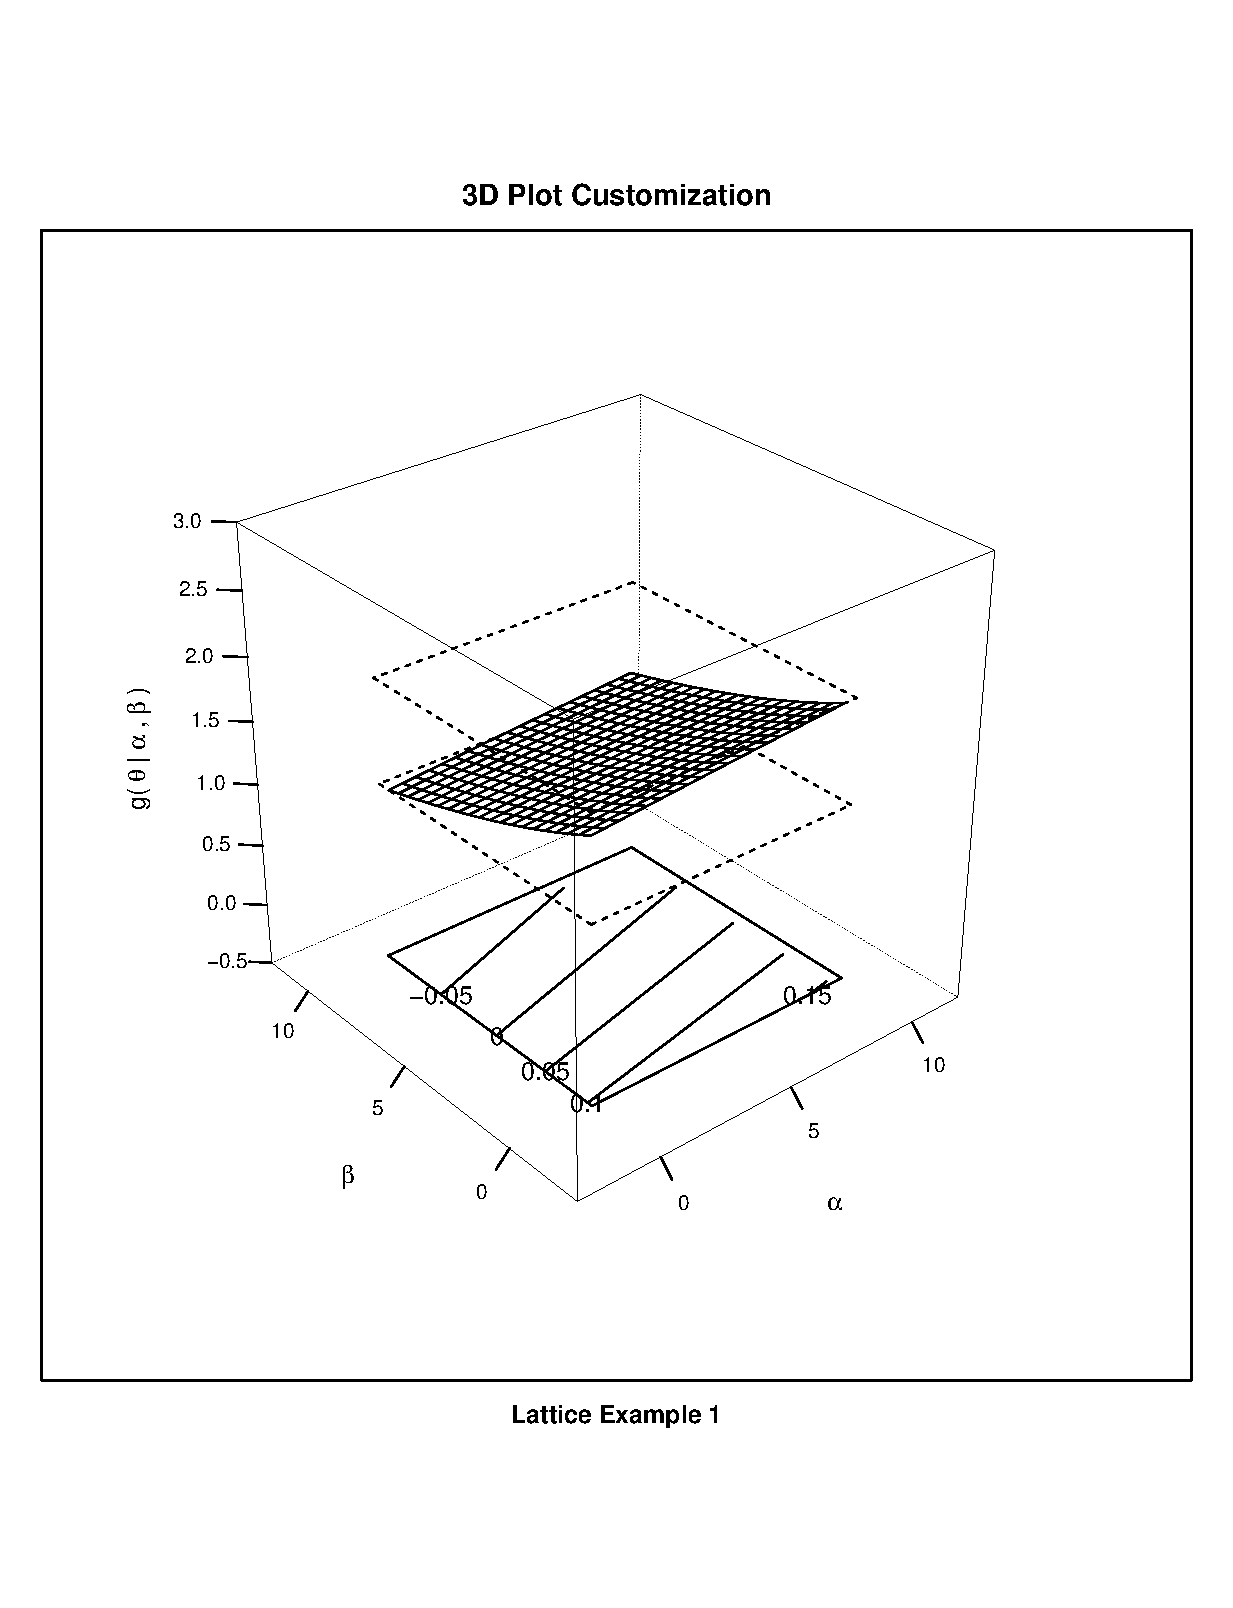
\includegraphics{./img/lattice-fig.eps}


\item \LaTeX 의 문서에 포함될 \texttt{.eps} 그래픽을 \texttt{R}에서 뽑았을 때는 아무런 문제가 없어 보였는데, 정작 \texttt{pdf}로 문서를 뽑아 보니까 이 그래픽이 들어간 페이지가 90도로 돌아가 있거나 혹은 그래픽이 90도로 회전되어 있을 경우에는 아래와 같이 하면 됩니다.

\begin{Schunk}
 \begin{Sinput}
  postscript(file=``filename.eps'', onefile=FALSE, horizontal=FALSE)
 \end{Sinput}
\end{Schunk}

이 문제에 대한 출처는 \texttt{postscript} 도움말입니다.

이문제를 다른 방법으로도 해결할 수 있습니다.  (대충 서너개 더 있음).
\end{enumerate}

%%%%%%%%%%%%%%%%%%%%%%%%%%%%%%%%%%%%%%%%%%%%%%%%%%%%%%%%%%%%%%%%%%%%%%%%
%
% Utilities
%
%%%%%%%%%%%%%%%%%%%%%%%%%%%%%%%%%%%%%%%%%%%%%%%%%%%%%%%%%%%%%%%%%%%%%%%%

\section{데이터 입출력 및 파일관리 유틸리티}
\begin{enumerate}
\item \texttt{read.table} 계열의 함수를 이용하여 데이터를 불러올 때 첫번째 인자는 파일의 위치와 파일명이 입력된 문자열이어야 합니다.
그런데, 간혹 문법에서 틀린 점도 없고, 불러오고자 하는 데이터 파일도 올바른 파일경로에 위치하고 있음에도 불구하고,
데이터를 찾을 수 없다고 하는 경우가 있습니다.
이것은 내부적으로 파일경로에 띄어쓰기, 특수문자, 혹은 특수한 인코딩 등 다양한 이유로 인하여 파일경로가 올바르게 처리되지 않았기 때문입니다.
아래와 같은 방법으로 \texttt{read.table()} 함수 사용시 \texttt{file.choose()} 함수를 함께 사용하면 이러한 문제를 해결이 가능합니다.


\begin{Schunk}
\begin{Soutput}
mydata <- read.table(file.choose(), header=TRUE, sep=",")
\end{Soutput}
\end{Schunk}


\end{enumerate}


%%%%%%%%%%%%%%%%%%%%%%%%%%%%%%%%%%%%%%%%%%%%%%%%%%%%%%%%%%%%%%%%%%%%%%%%
%
% Miscellinous
%
%%%%%%%%%%%%%%%%%%%%%%%%%%%%%%%%%%%%%%%%%%%%%%%%%%%%%%%%%%%%%%%%%%%%%%%%

\section{기타내용들}
\begin{enumerate}
\item 불러오고자 하는 데이터의 인코딩이 UTF-8가 아닐때 이를 확인하고, 데이터를 올바르게 불러오기 위한 내용은 \url{http://lists.r-forge.r-project.org/pipermail/ihelp-urquestion/2013-April/000017.html} 를 읽어보시길 바랍니다.

\item \texttt{R}을 한국어가 아닌 영문으로 사용하고 싶습니다 (버전에 관계없이 일반적으로 통용되는 방법 - 윈도우즈 사용자에게 맞추어 작성됨).
이를 설정하는 방법에 대해서는 \url{http://lists.r-forge.r-project.org/pipermail/ihelp-urquestion/2013-April/000003.html} 을 읽어보시길 바랍니다.
\end{enumerate}

\end{document}
